\documentclass[twoside]{book}

% Packages required by doxygen
\usepackage{fixltx2e}
\usepackage{calc}
\usepackage{doxygen}
\usepackage[export]{adjustbox} % also loads graphicx
\usepackage{graphicx}
\usepackage[utf8]{inputenc}
\usepackage{makeidx}
\usepackage{multicol}
\usepackage{multirow}
\PassOptionsToPackage{warn}{textcomp}
\usepackage{textcomp}
\usepackage[nointegrals]{wasysym}
\usepackage[table]{xcolor}

% Font selection
\usepackage[T1]{fontenc}
\usepackage[scaled=.90]{helvet}
\usepackage{courier}
\usepackage{amssymb}
\usepackage{sectsty}
\renewcommand{\familydefault}{\sfdefault}
\allsectionsfont{%
  \fontseries{bc}\selectfont%
  \color{darkgray}%
}
\renewcommand{\DoxyLabelFont}{%
  \fontseries{bc}\selectfont%
  \color{darkgray}%
}
\newcommand{\+}{\discretionary{\mbox{\scriptsize$\hookleftarrow$}}{}{}}

% Page & text layout
\usepackage{geometry}
\geometry{%
  a4paper,%
  top=2.5cm,%
  bottom=2.5cm,%
  left=2.5cm,%
  right=2.5cm%
}
\tolerance=750
\hfuzz=15pt
\hbadness=750
\setlength{\emergencystretch}{15pt}
\setlength{\parindent}{0cm}
\setlength{\parskip}{3ex plus 2ex minus 2ex}
\makeatletter
\renewcommand{\paragraph}{%
  \@startsection{paragraph}{4}{0ex}{-1.0ex}{1.0ex}{%
    \normalfont\normalsize\bfseries\SS@parafont%
  }%
}
\renewcommand{\subparagraph}{%
  \@startsection{subparagraph}{5}{0ex}{-1.0ex}{1.0ex}{%
    \normalfont\normalsize\bfseries\SS@subparafont%
  }%
}
\makeatother

% Headers & footers
\usepackage{fancyhdr}
\pagestyle{fancyplain}
\fancyhead[LE]{\fancyplain{}{\bfseries\thepage}}
\fancyhead[CE]{\fancyplain{}{}}
\fancyhead[RE]{\fancyplain{}{\bfseries\leftmark}}
\fancyhead[LO]{\fancyplain{}{\bfseries\rightmark}}
\fancyhead[CO]{\fancyplain{}{}}
\fancyhead[RO]{\fancyplain{}{\bfseries\thepage}}
\fancyfoot[LE]{\fancyplain{}{}}
\fancyfoot[CE]{\fancyplain{}{}}
\fancyfoot[RE]{\fancyplain{}{\bfseries\scriptsize Generated by Doxygen }}
\fancyfoot[LO]{\fancyplain{}{\bfseries\scriptsize Generated by Doxygen }}
\fancyfoot[CO]{\fancyplain{}{}}
\fancyfoot[RO]{\fancyplain{}{}}
\renewcommand{\footrulewidth}{0.4pt}
\renewcommand{\chaptermark}[1]{%
  \markboth{#1}{}%
}
\renewcommand{\sectionmark}[1]{%
  \markright{\thesection\ #1}%
}

% Indices & bibliography
\usepackage{natbib}
\usepackage[titles]{tocloft}
\setcounter{tocdepth}{3}
\setcounter{secnumdepth}{5}
\makeindex

% Hyperlinks (required, but should be loaded last)
\usepackage{ifpdf}
\ifpdf
  \usepackage[pdftex,pagebackref=true]{hyperref}
\else
  \usepackage[ps2pdf,pagebackref=true]{hyperref}
\fi
\hypersetup{%
  colorlinks=true,%
  linkcolor=blue,%
  citecolor=blue,%
  unicode%
}

% Custom commands
\newcommand{\clearemptydoublepage}{%
  \newpage{\pagestyle{empty}\cleardoublepage}%
}

\usepackage{caption}
\captionsetup{labelsep=space,justification=centering,font={bf},singlelinecheck=off,skip=4pt,position=top}

%===== C O N T E N T S =====

\begin{document}

% Titlepage & ToC
\hypersetup{pageanchor=false,
             bookmarksnumbered=true,
             pdfencoding=unicode
            }
\pagenumbering{alph}
\begin{titlepage}
\vspace*{7cm}
\begin{center}%
{\Large My Project }\\
\vspace*{1cm}
{\large Generated by Doxygen 1.8.14}\\
\end{center}
\end{titlepage}
\clearemptydoublepage
\pagenumbering{roman}
\tableofcontents
\clearemptydoublepage
\pagenumbering{arabic}
\hypersetup{pageanchor=true}

%--- Begin generated contents ---
\chapter{This is the $\ast$$\ast$\+H\+O\+M\+E\+P\+A\+G\+E$\ast$$\ast$.}
\label{md_index}
\Hypertarget{md_index}
Refer to \href{http://daringfireball.net/projects/markdown/}{\tt Markdown} for how to write markdown files. \subsection*{Quick Start Notes\+:}


\begin{DoxyEnumerate}
\item Add images to {\itshape images} folder if the file is referencing an image. 
\end{DoxyEnumerate}
\chapter{You\+Tube\+Tracker}
\label{md__r_e_a_d_m_e}
\Hypertarget{md__r_e_a_d_m_e}
 \subsection*{Description}

\mbox{\hyperlink{namespace_you_tube_tracker}{You\+Tube\+Tracker}} is a window app which allows user to search for videos, play videos, create local playlists and acquire playlist duration. ~\newline
App uses {\bfseries Youtube Data Api v3} to search and aquire videos data (title, embed html, id, thumbnail url, duration). {\bfseries Local database} is used to store playlists and theirs videos.

\subsection*{Getting Started}


\begin{DoxyItemize}
\item Genarate Youtube Data Api key (instruction\+: \href{https://developers.google.com/youtube/v3/getting-started#intro}{\tt https\+://developers.\+google.\+com/youtube/v3/getting-\/started\#intro} ~\newline
section\+: Before you start first 3 steps), Outh 2.\+0 is not required.
\item In project main directory add file A\+P\+I\+\_\+key.\+txt with generated api key.
\end{DoxyItemize}

\subsection*{Authors}

Contributors names and contact info
\begin{DoxyItemize}
\item Kacper Synator (\href{https://github.com/KacperSynator}{\tt https\+://github.\+com/\+Kacper\+Synator})
\item Paweł Potoczek (\href{https://github.com/PPotoczek}{\tt https\+://github.\+com/\+P\+Potoczek})
\end{DoxyItemize}

\subsection*{License}

This project is licensed under the M\+IT License -\/ see the L\+I\+C\+E\+N\+SE file for details 
\chapter{Namespace Index}
\section{Namespace List}
Here is a list of all documented namespaces with brief descriptions\+:\begin{DoxyCompactList}
\item\contentsline{section}{\mbox{\hyperlink{namespace_you_tube_tracker}{You\+Tube\+Tracker}} }{\pageref{namespace_you_tube_tracker}}{}
\end{DoxyCompactList}

\chapter{Hierarchical Index}
\section{Class Hierarchy}
This inheritance list is sorted roughly, but not completely, alphabetically\+:\begin{DoxyCompactList}
\item Application\begin{DoxyCompactList}
\item \contentsline{section}{You\+Tube\+Tracker.\+App}{\pageref{class_you_tube_tracker_1_1_app}}{}
\end{DoxyCompactList}
\item \contentsline{section}{You\+Tube\+Tracker.\+List\+Box\+Item}{\pageref{class_you_tube_tracker_1_1_list_box_item}}{}
\item \contentsline{section}{You\+Tube\+Tracker.\+Youtube\+Tracker.\+Search\+Result}{\pageref{class_you_tube_tracker_1_1_youtube_tracker_1_1_search_result}}{}
\item \contentsline{section}{You\+Tube\+Tracker.\+Video\+Data}{\pageref{struct_you_tube_tracker_1_1_video_data}}{}
\item \contentsline{section}{You\+Tube\+Tracker.\+Youtube\+Tracker.\+Video\+Result}{\pageref{class_you_tube_tracker_1_1_youtube_tracker_1_1_video_result}}{}
\item Window\begin{DoxyCompactList}
\item \contentsline{section}{You\+Tube\+Tracker.\+Main\+Window}{\pageref{class_you_tube_tracker_1_1_main_window}}{}
\end{DoxyCompactList}
\item \contentsline{section}{You\+Tube\+Tracker.\+Youtube\+Tracker}{\pageref{class_you_tube_tracker_1_1_youtube_tracker}}{}
\end{DoxyCompactList}

\chapter{Class Index}
\section{Class List}
Here are the classes, structs, unions and interfaces with brief descriptions\+:\begin{DoxyCompactList}
\item\contentsline{section}{\mbox{\hyperlink{class_you_tube_tracker_1_1_app}{You\+Tube\+Tracker.\+App}} \\*Logic interaction for class App.\+xaml }{\pageref{class_you_tube_tracker_1_1_app}}{}
\item\contentsline{section}{\mbox{\hyperlink{class_you_tube_tracker_1_1_list_box_item}{You\+Tube\+Tracker.\+List\+Box\+Item}} \\*Class {\ttfamily \mbox{\hyperlink{class_you_tube_tracker_1_1_list_box_item}{List\+Box\+Item}}} models an item of custom List\+Box. }{\pageref{class_you_tube_tracker_1_1_list_box_item}}{}
\item\contentsline{section}{\mbox{\hyperlink{class_you_tube_tracker_1_1_main_window}{You\+Tube\+Tracker.\+Main\+Window}} \\*Interaction logic for class Main\+Window.\+xaml }{\pageref{class_you_tube_tracker_1_1_main_window}}{}
\item\contentsline{section}{\mbox{\hyperlink{class_you_tube_tracker_1_1_youtube_tracker_1_1_search_result}{You\+Tube\+Tracker.\+Youtube\+Tracker.\+Search\+Result}} \\*Class {\ttfamily \mbox{\hyperlink{class_you_tube_tracker_1_1_youtube_tracker_1_1_search_result}{Search\+Result}}} models result of youtube Search request. Result videos, channels, playlists are stored in adequate lists. }{\pageref{class_you_tube_tracker_1_1_youtube_tracker_1_1_search_result}}{}
\item\contentsline{section}{\mbox{\hyperlink{struct_you_tube_tracker_1_1_video_data}{You\+Tube\+Tracker.\+Video\+Data}} \\*Struct {\ttfamily \mbox{\hyperlink{struct_you_tube_tracker_1_1_video_data}{Video\+Data}}} models youtube video\textquotesingle{}s data. }{\pageref{struct_you_tube_tracker_1_1_video_data}}{}
\item\contentsline{section}{\mbox{\hyperlink{class_you_tube_tracker_1_1_youtube_tracker_1_1_video_result}{You\+Tube\+Tracker.\+Youtube\+Tracker.\+Video\+Result}} \\*Class {\ttfamily \mbox{\hyperlink{class_you_tube_tracker_1_1_youtube_tracker_1_1_video_result}{Video\+Result}}} models result of youtube Video\+List request. Result videos are stored in list {\ttfamily videos\+\_\+data}. }{\pageref{class_you_tube_tracker_1_1_youtube_tracker_1_1_video_result}}{}
\item\contentsline{section}{\mbox{\hyperlink{class_you_tube_tracker_1_1_youtube_tracker}{You\+Tube\+Tracker.\+Youtube\+Tracker}} \\*Class {\ttfamily \mbox{\hyperlink{class_you_tube_tracker_1_1_youtube_tracker}{Youtube\+Tracker}}} stores currently used videos and is a link beetween window app, Youtube data A\+PI and database. }{\pageref{class_you_tube_tracker_1_1_youtube_tracker}}{}
\end{DoxyCompactList}

\chapter{Namespace Documentation}
\hypertarget{namespace_you_tube_tracker}{}\section{You\+Tube\+Tracker Namespace Reference}
\label{namespace_you_tube_tracker}\index{You\+Tube\+Tracker@{You\+Tube\+Tracker}}
\subsection*{Classes}
\begin{DoxyCompactItemize}
\item 
class \mbox{\hyperlink{class_you_tube_tracker_1_1_app}{App}}
\begin{DoxyCompactList}\small\item\em Logic interaction for class App.\+xaml \end{DoxyCompactList}\item 
class \mbox{\hyperlink{class_you_tube_tracker_1_1_list_box_item}{List\+Box\+Item}}
\begin{DoxyCompactList}\small\item\em Class {\ttfamily \mbox{\hyperlink{class_you_tube_tracker_1_1_list_box_item}{List\+Box\+Item}}} models an item of custom List\+Box. \end{DoxyCompactList}\item 
class \mbox{\hyperlink{class_you_tube_tracker_1_1_main_window}{Main\+Window}}
\begin{DoxyCompactList}\small\item\em Interaction logic for class Main\+Window.\+xaml \end{DoxyCompactList}\item 
struct \mbox{\hyperlink{struct_you_tube_tracker_1_1_video_data}{Video\+Data}}
\begin{DoxyCompactList}\small\item\em Struct {\ttfamily \mbox{\hyperlink{struct_you_tube_tracker_1_1_video_data}{Video\+Data}}} models youtube video\textquotesingle{}s data. \end{DoxyCompactList}\item 
class \mbox{\hyperlink{class_you_tube_tracker_1_1_youtube_tracker}{Youtube\+Tracker}}
\begin{DoxyCompactList}\small\item\em Class {\ttfamily \mbox{\hyperlink{class_you_tube_tracker_1_1_youtube_tracker}{Youtube\+Tracker}}} stores currently used videos and is a link beetween window app, Youtube data A\+PI and database. \end{DoxyCompactList}\end{DoxyCompactItemize}

\chapter{Class Documentation}
\hypertarget{class_you_tube_tracker_1_1_app}{}\section{You\+Tube\+Tracker.\+App Class Reference}
\label{class_you_tube_tracker_1_1_app}\index{You\+Tube\+Tracker.\+App@{You\+Tube\+Tracker.\+App}}


Logic interaction for class App.\+xaml  


Inheritance diagram for You\+Tube\+Tracker.\+App\+:\begin{figure}[H]
\begin{center}
\leavevmode
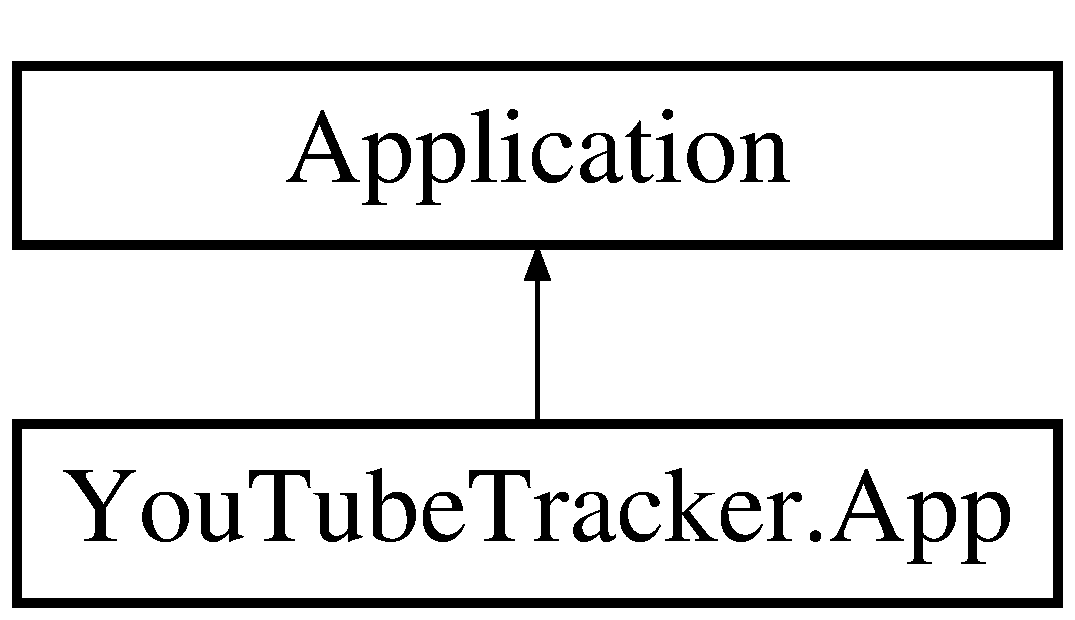
\includegraphics[height=2.000000cm]{class_you_tube_tracker_1_1_app}
\end{center}
\end{figure}
\subsection*{Properties}
\begin{DoxyCompactItemize}
\item 
static Data\+Base.\+Y\+Tracker\+D\+B\+Context \mbox{\hyperlink{class_you_tube_tracker_1_1_app_ac0a183370798e224e95ab6b5017de885}{Context}}\hspace{0.3cm}{\ttfamily  \mbox{[}get\mbox{]}}
\begin{DoxyCompactList}\small\item\em Returns database context {\ttfamily D\+B\+Context}. \end{DoxyCompactList}\end{DoxyCompactItemize}


\subsection{Detailed Description}
Logic interaction for class App.\+xaml 



\subsection{Property Documentation}
\mbox{\Hypertarget{class_you_tube_tracker_1_1_app_ac0a183370798e224e95ab6b5017de885}\label{class_you_tube_tracker_1_1_app_ac0a183370798e224e95ab6b5017de885}} 
\index{You\+Tube\+Tracker\+::\+App@{You\+Tube\+Tracker\+::\+App}!Context@{Context}}
\index{Context@{Context}!You\+Tube\+Tracker\+::\+App@{You\+Tube\+Tracker\+::\+App}}
\subsubsection{\texorpdfstring{Context}{Context}}
{\footnotesize\ttfamily Data\+Base.\+Y\+Tracker\+D\+B\+Context You\+Tube\+Tracker.\+App.\+Context\hspace{0.3cm}{\ttfamily [static]}, {\ttfamily [get]}}



Returns database context {\ttfamily D\+B\+Context}. 



The documentation for this class was generated from the following file\+:\begin{DoxyCompactItemize}
\item 
App.\+xaml.\+cs\end{DoxyCompactItemize}

\hypertarget{class_you_tube_tracker_1_1_list_box_item}{}\section{You\+Tube\+Tracker.\+List\+Box\+Item Class Reference}
\label{class_you_tube_tracker_1_1_list_box_item}\index{You\+Tube\+Tracker.\+List\+Box\+Item@{You\+Tube\+Tracker.\+List\+Box\+Item}}


Class {\ttfamily \mbox{\hyperlink{class_you_tube_tracker_1_1_list_box_item}{List\+Box\+Item}}} models an item of custom List\+Box.  


\subsection*{Public Member Functions}
\begin{DoxyCompactItemize}
\item 
\mbox{\hyperlink{class_you_tube_tracker_1_1_list_box_item_a4e0b02f68b5fa2dcb2e9181897f72495}{List\+Box\+Item}} (string \+\_\+text, string image\+\_\+url)
\begin{DoxyCompactList}\small\item\em Constructor for creating new item from text string and image url string. \end{DoxyCompactList}\end{DoxyCompactItemize}
\subsection*{Properties}
\begin{DoxyCompactItemize}
\item 
string \mbox{\hyperlink{class_you_tube_tracker_1_1_list_box_item_a39c781719df70576a81d8c16a524f946}{text}}\hspace{0.3cm}{\ttfamily  \mbox{[}get, set\mbox{]}}
\begin{DoxyCompactList}\small\item\em Text shown in Text\+Block. \end{DoxyCompactList}\item 
Uri \mbox{\hyperlink{class_you_tube_tracker_1_1_list_box_item_acb47893bd730bdc88d79198bbfd0b9bb}{image}}\hspace{0.3cm}{\ttfamily  \mbox{[}get, set\mbox{]}}
\begin{DoxyCompactList}\small\item\em Image displayed in Image. \end{DoxyCompactList}\end{DoxyCompactItemize}


\subsection{Detailed Description}
Class {\ttfamily \mbox{\hyperlink{class_you_tube_tracker_1_1_list_box_item}{List\+Box\+Item}}} models an item of custom List\+Box. 



\subsection{Constructor \& Destructor Documentation}
\mbox{\Hypertarget{class_you_tube_tracker_1_1_list_box_item_a4e0b02f68b5fa2dcb2e9181897f72495}\label{class_you_tube_tracker_1_1_list_box_item_a4e0b02f68b5fa2dcb2e9181897f72495}} 
\index{You\+Tube\+Tracker\+::\+List\+Box\+Item@{You\+Tube\+Tracker\+::\+List\+Box\+Item}!List\+Box\+Item@{List\+Box\+Item}}
\index{List\+Box\+Item@{List\+Box\+Item}!You\+Tube\+Tracker\+::\+List\+Box\+Item@{You\+Tube\+Tracker\+::\+List\+Box\+Item}}
\subsubsection{\texorpdfstring{List\+Box\+Item()}{ListBoxItem()}}
{\footnotesize\ttfamily You\+Tube\+Tracker.\+List\+Box\+Item.\+List\+Box\+Item (\begin{DoxyParamCaption}\item[{string}]{\+\_\+text,  }\item[{string}]{image\+\_\+url }\end{DoxyParamCaption})\hspace{0.3cm}{\ttfamily [inline]}}



Constructor for creating new item from text string and image url string. 


\begin{DoxyParams}{Parameters}
{\em \+\_\+text} & Text\\
\hline
{\em image\+\_\+url} & Image url\\
\hline
\end{DoxyParams}


\subsection{Property Documentation}
\mbox{\Hypertarget{class_you_tube_tracker_1_1_list_box_item_acb47893bd730bdc88d79198bbfd0b9bb}\label{class_you_tube_tracker_1_1_list_box_item_acb47893bd730bdc88d79198bbfd0b9bb}} 
\index{You\+Tube\+Tracker\+::\+List\+Box\+Item@{You\+Tube\+Tracker\+::\+List\+Box\+Item}!image@{image}}
\index{image@{image}!You\+Tube\+Tracker\+::\+List\+Box\+Item@{You\+Tube\+Tracker\+::\+List\+Box\+Item}}
\subsubsection{\texorpdfstring{image}{image}}
{\footnotesize\ttfamily Uri You\+Tube\+Tracker.\+List\+Box\+Item.\+image\hspace{0.3cm}{\ttfamily [get]}, {\ttfamily [set]}}



Image displayed in Image. 

\mbox{\Hypertarget{class_you_tube_tracker_1_1_list_box_item_a39c781719df70576a81d8c16a524f946}\label{class_you_tube_tracker_1_1_list_box_item_a39c781719df70576a81d8c16a524f946}} 
\index{You\+Tube\+Tracker\+::\+List\+Box\+Item@{You\+Tube\+Tracker\+::\+List\+Box\+Item}!text@{text}}
\index{text@{text}!You\+Tube\+Tracker\+::\+List\+Box\+Item@{You\+Tube\+Tracker\+::\+List\+Box\+Item}}
\subsubsection{\texorpdfstring{text}{text}}
{\footnotesize\ttfamily string You\+Tube\+Tracker.\+List\+Box\+Item.\+text\hspace{0.3cm}{\ttfamily [get]}, {\ttfamily [set]}}



Text shown in Text\+Block. 



The documentation for this class was generated from the following file\+:\begin{DoxyCompactItemize}
\item 
List\+Box\+Item.\+cs\end{DoxyCompactItemize}

\hypertarget{class_you_tube_tracker_1_1_main_window}{}\section{You\+Tube\+Tracker.\+Main\+Window Class Reference}
\label{class_you_tube_tracker_1_1_main_window}\index{You\+Tube\+Tracker.\+Main\+Window@{You\+Tube\+Tracker.\+Main\+Window}}


Interaction logic for class Main\+Window.\+xaml  


Inheritance diagram for You\+Tube\+Tracker.\+Main\+Window\+:\begin{figure}[H]
\begin{center}
\leavevmode
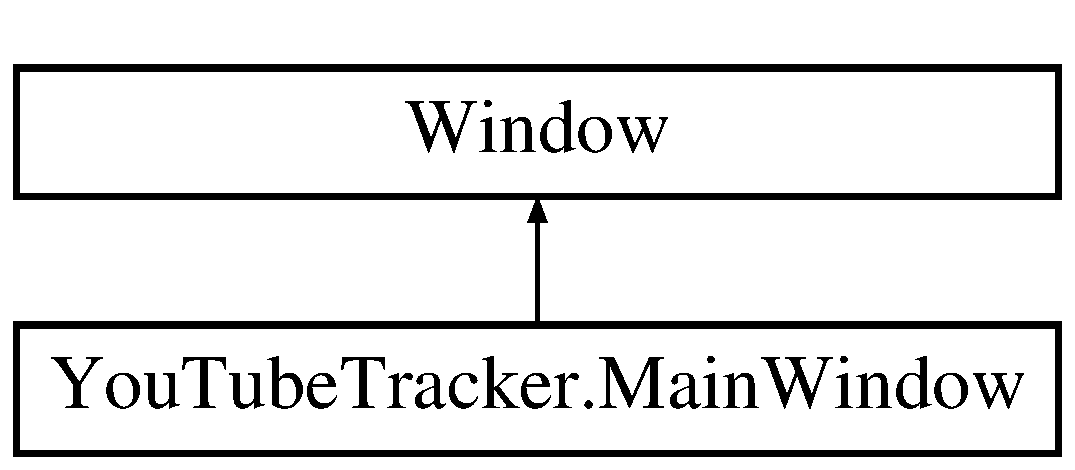
\includegraphics[height=2.000000cm]{class_you_tube_tracker_1_1_main_window}
\end{center}
\end{figure}
\subsection*{Public Member Functions}
\begin{DoxyCompactItemize}
\item 
\mbox{\hyperlink{class_you_tube_tracker_1_1_main_window_a1e4be9d4abe38411826ace3c9c9b6b06}{Main\+Window}} ()
\begin{DoxyCompactList}\small\item\em Initializes components and populates Combo\+Box\+: {\ttfamily play\+List\+CB}. \end{DoxyCompactList}\item 
void \mbox{\hyperlink{class_you_tube_tracker_1_1_main_window_aa1784f0a72b941e073f753939c5f89d5}{Update\+Playlist\+Combo\+Box}} ()
\begin{DoxyCompactList}\small\item\em Populates Combo\+Box\+: {\ttfamily play\+List\+CB} with database playlists\textquotesingle{} names. \end{DoxyCompactList}\item 
void \mbox{\hyperlink{class_you_tube_tracker_1_1_main_window_ae42b5a4f3b7d6e720ef2825f6786512d}{Update\+Video\+List\+Box}} (List$<$ \mbox{\hyperlink{struct_you_tube_tracker_1_1_video_data}{Video\+Data}} $>$ videos)
\begin{DoxyCompactList}\small\item\em Updates List\+Box\+: {\ttfamily video\+List\+Box} with given list of videos. \end{DoxyCompactList}\item 
void \mbox{\hyperlink{class_you_tube_tracker_1_1_main_window_a0f16b6bca0c659f84e23615a938fc3b5}{Update\+Playlist\+Info\+Text\+Block}} (int playlist\+\_\+id)
\begin{DoxyCompactList}\small\item\em Update Text\+Block\+: {\ttfamily playlist\+Info} with given playlist info. \end{DoxyCompactList}\end{DoxyCompactItemize}


\subsection{Detailed Description}
Interaction logic for class Main\+Window.\+xaml 



\subsection{Constructor \& Destructor Documentation}
\mbox{\Hypertarget{class_you_tube_tracker_1_1_main_window_a1e4be9d4abe38411826ace3c9c9b6b06}\label{class_you_tube_tracker_1_1_main_window_a1e4be9d4abe38411826ace3c9c9b6b06}} 
\index{You\+Tube\+Tracker\+::\+Main\+Window@{You\+Tube\+Tracker\+::\+Main\+Window}!Main\+Window@{Main\+Window}}
\index{Main\+Window@{Main\+Window}!You\+Tube\+Tracker\+::\+Main\+Window@{You\+Tube\+Tracker\+::\+Main\+Window}}
\subsubsection{\texorpdfstring{Main\+Window()}{MainWindow()}}
{\footnotesize\ttfamily You\+Tube\+Tracker.\+Main\+Window.\+Main\+Window (\begin{DoxyParamCaption}{ }\end{DoxyParamCaption})\hspace{0.3cm}{\ttfamily [inline]}}



Initializes components and populates Combo\+Box\+: {\ttfamily play\+List\+CB}. 



\subsection{Member Function Documentation}
\mbox{\Hypertarget{class_you_tube_tracker_1_1_main_window_aa1784f0a72b941e073f753939c5f89d5}\label{class_you_tube_tracker_1_1_main_window_aa1784f0a72b941e073f753939c5f89d5}} 
\index{You\+Tube\+Tracker\+::\+Main\+Window@{You\+Tube\+Tracker\+::\+Main\+Window}!Update\+Playlist\+Combo\+Box@{Update\+Playlist\+Combo\+Box}}
\index{Update\+Playlist\+Combo\+Box@{Update\+Playlist\+Combo\+Box}!You\+Tube\+Tracker\+::\+Main\+Window@{You\+Tube\+Tracker\+::\+Main\+Window}}
\subsubsection{\texorpdfstring{Update\+Playlist\+Combo\+Box()}{UpdatePlaylistComboBox()}}
{\footnotesize\ttfamily void You\+Tube\+Tracker.\+Main\+Window.\+Update\+Playlist\+Combo\+Box (\begin{DoxyParamCaption}{ }\end{DoxyParamCaption})\hspace{0.3cm}{\ttfamily [inline]}}



Populates Combo\+Box\+: {\ttfamily play\+List\+CB} with database playlists\textquotesingle{} names. 

\mbox{\Hypertarget{class_you_tube_tracker_1_1_main_window_a0f16b6bca0c659f84e23615a938fc3b5}\label{class_you_tube_tracker_1_1_main_window_a0f16b6bca0c659f84e23615a938fc3b5}} 
\index{You\+Tube\+Tracker\+::\+Main\+Window@{You\+Tube\+Tracker\+::\+Main\+Window}!Update\+Playlist\+Info\+Text\+Block@{Update\+Playlist\+Info\+Text\+Block}}
\index{Update\+Playlist\+Info\+Text\+Block@{Update\+Playlist\+Info\+Text\+Block}!You\+Tube\+Tracker\+::\+Main\+Window@{You\+Tube\+Tracker\+::\+Main\+Window}}
\subsubsection{\texorpdfstring{Update\+Playlist\+Info\+Text\+Block()}{UpdatePlaylistInfoTextBlock()}}
{\footnotesize\ttfamily void You\+Tube\+Tracker.\+Main\+Window.\+Update\+Playlist\+Info\+Text\+Block (\begin{DoxyParamCaption}\item[{int}]{playlist\+\_\+id }\end{DoxyParamCaption})\hspace{0.3cm}{\ttfamily [inline]}}



Update Text\+Block\+: {\ttfamily playlist\+Info} with given playlist info. 


\begin{DoxyParams}{Parameters}
{\em playlist\+\_\+id} & Playlist id\\
\hline
\end{DoxyParams}
\mbox{\Hypertarget{class_you_tube_tracker_1_1_main_window_ae42b5a4f3b7d6e720ef2825f6786512d}\label{class_you_tube_tracker_1_1_main_window_ae42b5a4f3b7d6e720ef2825f6786512d}} 
\index{You\+Tube\+Tracker\+::\+Main\+Window@{You\+Tube\+Tracker\+::\+Main\+Window}!Update\+Video\+List\+Box@{Update\+Video\+List\+Box}}
\index{Update\+Video\+List\+Box@{Update\+Video\+List\+Box}!You\+Tube\+Tracker\+::\+Main\+Window@{You\+Tube\+Tracker\+::\+Main\+Window}}
\subsubsection{\texorpdfstring{Update\+Video\+List\+Box()}{UpdateVideoListBox()}}
{\footnotesize\ttfamily void You\+Tube\+Tracker.\+Main\+Window.\+Update\+Video\+List\+Box (\begin{DoxyParamCaption}\item[{List$<$ \mbox{\hyperlink{struct_you_tube_tracker_1_1_video_data}{Video\+Data}} $>$}]{videos }\end{DoxyParamCaption})\hspace{0.3cm}{\ttfamily [inline]}}



Updates List\+Box\+: {\ttfamily video\+List\+Box} with given list of videos. 


\begin{DoxyParams}{Parameters}
{\em videos} & List of videos\\
\hline
\end{DoxyParams}


The documentation for this class was generated from the following file\+:\begin{DoxyCompactItemize}
\item 
Main\+Window.\+xaml.\+cs\end{DoxyCompactItemize}

\hypertarget{class_you_tube_tracker_1_1_youtube_tracker_1_1_search_result}{}\section{You\+Tube\+Tracker.\+Youtube\+Tracker.\+Search\+Result Class Reference}
\label{class_you_tube_tracker_1_1_youtube_tracker_1_1_search_result}\index{You\+Tube\+Tracker.\+Youtube\+Tracker.\+Search\+Result@{You\+Tube\+Tracker.\+Youtube\+Tracker.\+Search\+Result}}


Class {\ttfamily \mbox{\hyperlink{class_you_tube_tracker_1_1_youtube_tracker_1_1_search_result}{Search\+Result}}} models result of youtube Search request. Result videos, channels, playlists are stored in adequate lists.  


\subsection*{Public Member Functions}
\begin{DoxyCompactItemize}
\item 
\mbox{\hyperlink{class_you_tube_tracker_1_1_youtube_tracker_1_1_search_result_a14c8dd3872fb03f75075f6b311f64694}{Search\+Result}} ()
\begin{DoxyCompactList}\small\item\em Parameterless constructor. \end{DoxyCompactList}\end{DoxyCompactItemize}
\subsection*{Public Attributes}
\begin{DoxyCompactItemize}
\item 
List$<$ \mbox{\hyperlink{struct_you_tube_tracker_1_1_video_data}{Video\+Data}} $>$ \mbox{\hyperlink{class_you_tube_tracker_1_1_youtube_tracker_1_1_search_result_a59c445d69a5f87735ddb589d7e3be7f8}{videos}}
\begin{DoxyCompactList}\small\item\em Search videos results. \end{DoxyCompactList}\item 
List$<$ \mbox{\hyperlink{struct_you_tube_tracker_1_1_video_data}{Video\+Data}} $>$ \mbox{\hyperlink{class_you_tube_tracker_1_1_youtube_tracker_1_1_search_result_a1edc3536b63100ee775fa1c7ab5f6569}{channels}}
\begin{DoxyCompactList}\small\item\em Search channels results. \end{DoxyCompactList}\item 
List$<$ \mbox{\hyperlink{struct_you_tube_tracker_1_1_video_data}{Video\+Data}} $>$ \mbox{\hyperlink{class_you_tube_tracker_1_1_youtube_tracker_1_1_search_result_a4d9162b386c247731a23d8c44934fdbf}{playlists}}
\begin{DoxyCompactList}\small\item\em Search playlists results. \end{DoxyCompactList}\end{DoxyCompactItemize}


\subsection{Detailed Description}
Class {\ttfamily \mbox{\hyperlink{class_you_tube_tracker_1_1_youtube_tracker_1_1_search_result}{Search\+Result}}} models result of youtube Search request. Result videos, channels, playlists are stored in adequate lists. 



\subsection{Constructor \& Destructor Documentation}
\mbox{\Hypertarget{class_you_tube_tracker_1_1_youtube_tracker_1_1_search_result_a14c8dd3872fb03f75075f6b311f64694}\label{class_you_tube_tracker_1_1_youtube_tracker_1_1_search_result_a14c8dd3872fb03f75075f6b311f64694}} 
\index{You\+Tube\+Tracker\+::\+Youtube\+Tracker\+::\+Search\+Result@{You\+Tube\+Tracker\+::\+Youtube\+Tracker\+::\+Search\+Result}!Search\+Result@{Search\+Result}}
\index{Search\+Result@{Search\+Result}!You\+Tube\+Tracker\+::\+Youtube\+Tracker\+::\+Search\+Result@{You\+Tube\+Tracker\+::\+Youtube\+Tracker\+::\+Search\+Result}}
\subsubsection{\texorpdfstring{Search\+Result()}{SearchResult()}}
{\footnotesize\ttfamily You\+Tube\+Tracker.\+Youtube\+Tracker.\+Search\+Result.\+Search\+Result (\begin{DoxyParamCaption}{ }\end{DoxyParamCaption})\hspace{0.3cm}{\ttfamily [inline]}}



Parameterless constructor. 



\subsection{Member Data Documentation}
\mbox{\Hypertarget{class_you_tube_tracker_1_1_youtube_tracker_1_1_search_result_a1edc3536b63100ee775fa1c7ab5f6569}\label{class_you_tube_tracker_1_1_youtube_tracker_1_1_search_result_a1edc3536b63100ee775fa1c7ab5f6569}} 
\index{You\+Tube\+Tracker\+::\+Youtube\+Tracker\+::\+Search\+Result@{You\+Tube\+Tracker\+::\+Youtube\+Tracker\+::\+Search\+Result}!channels@{channels}}
\index{channels@{channels}!You\+Tube\+Tracker\+::\+Youtube\+Tracker\+::\+Search\+Result@{You\+Tube\+Tracker\+::\+Youtube\+Tracker\+::\+Search\+Result}}
\subsubsection{\texorpdfstring{channels}{channels}}
{\footnotesize\ttfamily List$<$\mbox{\hyperlink{struct_you_tube_tracker_1_1_video_data}{Video\+Data}}$>$ You\+Tube\+Tracker.\+Youtube\+Tracker.\+Search\+Result.\+channels}



Search channels results. 

\mbox{\Hypertarget{class_you_tube_tracker_1_1_youtube_tracker_1_1_search_result_a4d9162b386c247731a23d8c44934fdbf}\label{class_you_tube_tracker_1_1_youtube_tracker_1_1_search_result_a4d9162b386c247731a23d8c44934fdbf}} 
\index{You\+Tube\+Tracker\+::\+Youtube\+Tracker\+::\+Search\+Result@{You\+Tube\+Tracker\+::\+Youtube\+Tracker\+::\+Search\+Result}!playlists@{playlists}}
\index{playlists@{playlists}!You\+Tube\+Tracker\+::\+Youtube\+Tracker\+::\+Search\+Result@{You\+Tube\+Tracker\+::\+Youtube\+Tracker\+::\+Search\+Result}}
\subsubsection{\texorpdfstring{playlists}{playlists}}
{\footnotesize\ttfamily List$<$\mbox{\hyperlink{struct_you_tube_tracker_1_1_video_data}{Video\+Data}}$>$ You\+Tube\+Tracker.\+Youtube\+Tracker.\+Search\+Result.\+playlists}



Search playlists results. 

\mbox{\Hypertarget{class_you_tube_tracker_1_1_youtube_tracker_1_1_search_result_a59c445d69a5f87735ddb589d7e3be7f8}\label{class_you_tube_tracker_1_1_youtube_tracker_1_1_search_result_a59c445d69a5f87735ddb589d7e3be7f8}} 
\index{You\+Tube\+Tracker\+::\+Youtube\+Tracker\+::\+Search\+Result@{You\+Tube\+Tracker\+::\+Youtube\+Tracker\+::\+Search\+Result}!videos@{videos}}
\index{videos@{videos}!You\+Tube\+Tracker\+::\+Youtube\+Tracker\+::\+Search\+Result@{You\+Tube\+Tracker\+::\+Youtube\+Tracker\+::\+Search\+Result}}
\subsubsection{\texorpdfstring{videos}{videos}}
{\footnotesize\ttfamily List$<$\mbox{\hyperlink{struct_you_tube_tracker_1_1_video_data}{Video\+Data}}$>$ You\+Tube\+Tracker.\+Youtube\+Tracker.\+Search\+Result.\+videos}



Search videos results. 



The documentation for this class was generated from the following file\+:\begin{DoxyCompactItemize}
\item 
Youtube\+Search.\+cs\end{DoxyCompactItemize}

\hypertarget{struct_you_tube_tracker_1_1_video_data}{}\section{You\+Tube\+Tracker.\+Video\+Data Struct Reference}
\label{struct_you_tube_tracker_1_1_video_data}\index{You\+Tube\+Tracker.\+Video\+Data@{You\+Tube\+Tracker.\+Video\+Data}}


Struct {\ttfamily \mbox{\hyperlink{struct_you_tube_tracker_1_1_video_data}{Video\+Data}}} models youtube video\textquotesingle{}s data.  


\subsection*{Public Member Functions}
\begin{DoxyCompactItemize}
\item 
\mbox{\hyperlink{struct_you_tube_tracker_1_1_video_data_ae0bc57a279eeef5070b17086d2a7bcc2}{Video\+Data}} (string \+\_\+id)
\begin{DoxyCompactList}\small\item\em Constructs a new instance using only id, rest set to empty string. \end{DoxyCompactList}\item 
\mbox{\hyperlink{struct_you_tube_tracker_1_1_video_data_a5bd160817cfc9b4671d344f9a25b8277}{Video\+Data}} (string \+\_\+id, string \+\_\+title, string \+\_\+duration, string \+\_\+embed\+\_\+html, string \+\_\+thumbnail\+\_\+url)
\begin{DoxyCompactList}\small\item\em Full parameter constructor \end{DoxyCompactList}\end{DoxyCompactItemize}
\subsection*{Properties}
\begin{DoxyCompactItemize}
\item 
string \mbox{\hyperlink{struct_you_tube_tracker_1_1_video_data_a82645a050c3eb08fa1a69fbaaf80a149}{id}}\hspace{0.3cm}{\ttfamily  \mbox{[}get, set\mbox{]}}
\begin{DoxyCompactList}\small\item\em Youtube vido id \end{DoxyCompactList}\item 
string \mbox{\hyperlink{struct_you_tube_tracker_1_1_video_data_a27e67b8b39d459a7fb2107ab4ef7fdd7}{title}}\hspace{0.3cm}{\ttfamily  \mbox{[}get, set\mbox{]}}
\begin{DoxyCompactList}\small\item\em Title of video \end{DoxyCompactList}\item 
string \mbox{\hyperlink{struct_you_tube_tracker_1_1_video_data_a2e068777a3633b83e7300d84d8a1d3e3}{thumbnail\+\_\+url}}\hspace{0.3cm}{\ttfamily  \mbox{[}get, set\mbox{]}}
\begin{DoxyCompactList}\small\item\em Thumbnai url, image \end{DoxyCompactList}\item 
string \mbox{\hyperlink{struct_you_tube_tracker_1_1_video_data_a77293a0d3f3fde7099a415f488d96885}{duration}}\hspace{0.3cm}{\ttfamily  \mbox{[}get, set\mbox{]}}
\begin{DoxyCompactList}\small\item\em Duration of video \end{DoxyCompactList}\item 
string \mbox{\hyperlink{struct_you_tube_tracker_1_1_video_data_ae6fbc40e0ecdce522c2a65f68fba43c9}{embed\+\_\+html}}\hspace{0.3cm}{\ttfamily  \mbox{[}get, set\mbox{]}}
\begin{DoxyCompactList}\small\item\em Videos\textquotesingle{}s embed html for playing a video in web browser. \end{DoxyCompactList}\end{DoxyCompactItemize}


\subsection{Detailed Description}
Struct {\ttfamily \mbox{\hyperlink{struct_you_tube_tracker_1_1_video_data}{Video\+Data}}} models youtube video\textquotesingle{}s data. 



\subsection{Constructor \& Destructor Documentation}
\mbox{\Hypertarget{struct_you_tube_tracker_1_1_video_data_ae0bc57a279eeef5070b17086d2a7bcc2}\label{struct_you_tube_tracker_1_1_video_data_ae0bc57a279eeef5070b17086d2a7bcc2}} 
\index{You\+Tube\+Tracker\+::\+Video\+Data@{You\+Tube\+Tracker\+::\+Video\+Data}!Video\+Data@{Video\+Data}}
\index{Video\+Data@{Video\+Data}!You\+Tube\+Tracker\+::\+Video\+Data@{You\+Tube\+Tracker\+::\+Video\+Data}}
\subsubsection{\texorpdfstring{Video\+Data()}{VideoData()}\hspace{0.1cm}{\footnotesize\ttfamily [1/2]}}
{\footnotesize\ttfamily You\+Tube\+Tracker.\+Video\+Data.\+Video\+Data (\begin{DoxyParamCaption}\item[{string}]{\+\_\+id }\end{DoxyParamCaption})\hspace{0.3cm}{\ttfamily [inline]}}



Constructs a new instance using only id, rest set to empty string. 


\begin{DoxyParams}{Parameters}
{\em \+\_\+id} & Video\textquotesingle{}s youtube id\\
\hline
\end{DoxyParams}
\mbox{\Hypertarget{struct_you_tube_tracker_1_1_video_data_a5bd160817cfc9b4671d344f9a25b8277}\label{struct_you_tube_tracker_1_1_video_data_a5bd160817cfc9b4671d344f9a25b8277}} 
\index{You\+Tube\+Tracker\+::\+Video\+Data@{You\+Tube\+Tracker\+::\+Video\+Data}!Video\+Data@{Video\+Data}}
\index{Video\+Data@{Video\+Data}!You\+Tube\+Tracker\+::\+Video\+Data@{You\+Tube\+Tracker\+::\+Video\+Data}}
\subsubsection{\texorpdfstring{Video\+Data()}{VideoData()}\hspace{0.1cm}{\footnotesize\ttfamily [2/2]}}
{\footnotesize\ttfamily You\+Tube\+Tracker.\+Video\+Data.\+Video\+Data (\begin{DoxyParamCaption}\item[{string}]{\+\_\+id,  }\item[{string}]{\+\_\+title,  }\item[{string}]{\+\_\+duration,  }\item[{string}]{\+\_\+embed\+\_\+html,  }\item[{string}]{\+\_\+thumbnail\+\_\+url }\end{DoxyParamCaption})\hspace{0.3cm}{\ttfamily [inline]}}



Full parameter constructor 


\begin{DoxyParams}{Parameters}
{\em \+\_\+id} & Video\textquotesingle{}s youtube id\\
\hline
{\em \+\_\+title} & Video\textquotesingle{}s title\\
\hline
{\em \+\_\+duration} & Video\textquotesingle{}s duration\\
\hline
{\em \+\_\+embed\+\_\+html} & Video\textquotesingle{}s embed html\\
\hline
{\em \+\_\+thumbnail\+\_\+url} & Video\textquotesingle{}s thumbnail url\\
\hline
\end{DoxyParams}


\subsection{Property Documentation}
\mbox{\Hypertarget{struct_you_tube_tracker_1_1_video_data_a77293a0d3f3fde7099a415f488d96885}\label{struct_you_tube_tracker_1_1_video_data_a77293a0d3f3fde7099a415f488d96885}} 
\index{You\+Tube\+Tracker\+::\+Video\+Data@{You\+Tube\+Tracker\+::\+Video\+Data}!duration@{duration}}
\index{duration@{duration}!You\+Tube\+Tracker\+::\+Video\+Data@{You\+Tube\+Tracker\+::\+Video\+Data}}
\subsubsection{\texorpdfstring{duration}{duration}}
{\footnotesize\ttfamily string You\+Tube\+Tracker.\+Video\+Data.\+duration\hspace{0.3cm}{\ttfamily [get]}, {\ttfamily [set]}}



Duration of video 

\mbox{\Hypertarget{struct_you_tube_tracker_1_1_video_data_ae6fbc40e0ecdce522c2a65f68fba43c9}\label{struct_you_tube_tracker_1_1_video_data_ae6fbc40e0ecdce522c2a65f68fba43c9}} 
\index{You\+Tube\+Tracker\+::\+Video\+Data@{You\+Tube\+Tracker\+::\+Video\+Data}!embed\+\_\+html@{embed\+\_\+html}}
\index{embed\+\_\+html@{embed\+\_\+html}!You\+Tube\+Tracker\+::\+Video\+Data@{You\+Tube\+Tracker\+::\+Video\+Data}}
\subsubsection{\texorpdfstring{embed\+\_\+html}{embed\_html}}
{\footnotesize\ttfamily string You\+Tube\+Tracker.\+Video\+Data.\+embed\+\_\+html\hspace{0.3cm}{\ttfamily [get]}, {\ttfamily [set]}}



Videos\textquotesingle{}s embed html for playing a video in web browser. 

\mbox{\Hypertarget{struct_you_tube_tracker_1_1_video_data_a82645a050c3eb08fa1a69fbaaf80a149}\label{struct_you_tube_tracker_1_1_video_data_a82645a050c3eb08fa1a69fbaaf80a149}} 
\index{You\+Tube\+Tracker\+::\+Video\+Data@{You\+Tube\+Tracker\+::\+Video\+Data}!id@{id}}
\index{id@{id}!You\+Tube\+Tracker\+::\+Video\+Data@{You\+Tube\+Tracker\+::\+Video\+Data}}
\subsubsection{\texorpdfstring{id}{id}}
{\footnotesize\ttfamily string You\+Tube\+Tracker.\+Video\+Data.\+id\hspace{0.3cm}{\ttfamily [get]}, {\ttfamily [set]}}



Youtube vido id 

\mbox{\Hypertarget{struct_you_tube_tracker_1_1_video_data_a2e068777a3633b83e7300d84d8a1d3e3}\label{struct_you_tube_tracker_1_1_video_data_a2e068777a3633b83e7300d84d8a1d3e3}} 
\index{You\+Tube\+Tracker\+::\+Video\+Data@{You\+Tube\+Tracker\+::\+Video\+Data}!thumbnail\+\_\+url@{thumbnail\+\_\+url}}
\index{thumbnail\+\_\+url@{thumbnail\+\_\+url}!You\+Tube\+Tracker\+::\+Video\+Data@{You\+Tube\+Tracker\+::\+Video\+Data}}
\subsubsection{\texorpdfstring{thumbnail\+\_\+url}{thumbnail\_url}}
{\footnotesize\ttfamily string You\+Tube\+Tracker.\+Video\+Data.\+thumbnail\+\_\+url\hspace{0.3cm}{\ttfamily [get]}, {\ttfamily [set]}}



Thumbnai url, image 

\mbox{\Hypertarget{struct_you_tube_tracker_1_1_video_data_a27e67b8b39d459a7fb2107ab4ef7fdd7}\label{struct_you_tube_tracker_1_1_video_data_a27e67b8b39d459a7fb2107ab4ef7fdd7}} 
\index{You\+Tube\+Tracker\+::\+Video\+Data@{You\+Tube\+Tracker\+::\+Video\+Data}!title@{title}}
\index{title@{title}!You\+Tube\+Tracker\+::\+Video\+Data@{You\+Tube\+Tracker\+::\+Video\+Data}}
\subsubsection{\texorpdfstring{title}{title}}
{\footnotesize\ttfamily string You\+Tube\+Tracker.\+Video\+Data.\+title\hspace{0.3cm}{\ttfamily [get]}, {\ttfamily [set]}}



Title of video 



The documentation for this struct was generated from the following file\+:\begin{DoxyCompactItemize}
\item 
Video\+Data.\+cs\end{DoxyCompactItemize}

\hypertarget{class_you_tube_tracker_1_1_youtube_tracker_1_1_video_result}{}\section{You\+Tube\+Tracker.\+Youtube\+Tracker.\+Video\+Result Class Reference}
\label{class_you_tube_tracker_1_1_youtube_tracker_1_1_video_result}\index{You\+Tube\+Tracker.\+Youtube\+Tracker.\+Video\+Result@{You\+Tube\+Tracker.\+Youtube\+Tracker.\+Video\+Result}}


Class {\ttfamily \mbox{\hyperlink{class_you_tube_tracker_1_1_youtube_tracker_1_1_video_result}{Video\+Result}}} models result of youtube Video\+List request. Result videos are stored in list {\ttfamily videos\+\_\+data}.  


\subsection*{Public Member Functions}
\begin{DoxyCompactItemize}
\item 
\mbox{\hyperlink{class_you_tube_tracker_1_1_youtube_tracker_1_1_video_result_a6b681268664a1705f678db0444d0304b}{Video\+Result}} ()
\begin{DoxyCompactList}\small\item\em Parameterless constructor. \end{DoxyCompactList}\end{DoxyCompactItemize}
\subsection*{Public Attributes}
\begin{DoxyCompactItemize}
\item 
List$<$ \mbox{\hyperlink{struct_you_tube_tracker_1_1_video_data}{Video\+Data}} $>$ \mbox{\hyperlink{class_you_tube_tracker_1_1_youtube_tracker_1_1_video_result_a6939c5928302095e392762ace6454018}{videos\+\_\+data}}
\begin{DoxyCompactList}\small\item\em Video list result videos. \end{DoxyCompactList}\end{DoxyCompactItemize}


\subsection{Detailed Description}
Class {\ttfamily \mbox{\hyperlink{class_you_tube_tracker_1_1_youtube_tracker_1_1_video_result}{Video\+Result}}} models result of youtube Video\+List request. Result videos are stored in list {\ttfamily videos\+\_\+data}. 



\subsection{Constructor \& Destructor Documentation}
\mbox{\Hypertarget{class_you_tube_tracker_1_1_youtube_tracker_1_1_video_result_a6b681268664a1705f678db0444d0304b}\label{class_you_tube_tracker_1_1_youtube_tracker_1_1_video_result_a6b681268664a1705f678db0444d0304b}} 
\index{You\+Tube\+Tracker\+::\+Youtube\+Tracker\+::\+Video\+Result@{You\+Tube\+Tracker\+::\+Youtube\+Tracker\+::\+Video\+Result}!Video\+Result@{Video\+Result}}
\index{Video\+Result@{Video\+Result}!You\+Tube\+Tracker\+::\+Youtube\+Tracker\+::\+Video\+Result@{You\+Tube\+Tracker\+::\+Youtube\+Tracker\+::\+Video\+Result}}
\subsubsection{\texorpdfstring{Video\+Result()}{VideoResult()}}
{\footnotesize\ttfamily You\+Tube\+Tracker.\+Youtube\+Tracker.\+Video\+Result.\+Video\+Result (\begin{DoxyParamCaption}{ }\end{DoxyParamCaption})\hspace{0.3cm}{\ttfamily [inline]}}



Parameterless constructor. 



\subsection{Member Data Documentation}
\mbox{\Hypertarget{class_you_tube_tracker_1_1_youtube_tracker_1_1_video_result_a6939c5928302095e392762ace6454018}\label{class_you_tube_tracker_1_1_youtube_tracker_1_1_video_result_a6939c5928302095e392762ace6454018}} 
\index{You\+Tube\+Tracker\+::\+Youtube\+Tracker\+::\+Video\+Result@{You\+Tube\+Tracker\+::\+Youtube\+Tracker\+::\+Video\+Result}!videos\+\_\+data@{videos\+\_\+data}}
\index{videos\+\_\+data@{videos\+\_\+data}!You\+Tube\+Tracker\+::\+Youtube\+Tracker\+::\+Video\+Result@{You\+Tube\+Tracker\+::\+Youtube\+Tracker\+::\+Video\+Result}}
\subsubsection{\texorpdfstring{videos\+\_\+data}{videos\_data}}
{\footnotesize\ttfamily List$<$\mbox{\hyperlink{struct_you_tube_tracker_1_1_video_data}{Video\+Data}}$>$ You\+Tube\+Tracker.\+Youtube\+Tracker.\+Video\+Result.\+videos\+\_\+data}



Video list result videos. 



The documentation for this class was generated from the following file\+:\begin{DoxyCompactItemize}
\item 
Youtube\+Video.\+cs\end{DoxyCompactItemize}

\hypertarget{class_you_tube_tracker_1_1_youtube_tracker}{}\section{You\+Tube\+Tracker.\+Youtube\+Tracker Class Reference}
\label{class_you_tube_tracker_1_1_youtube_tracker}\index{You\+Tube\+Tracker.\+Youtube\+Tracker@{You\+Tube\+Tracker.\+Youtube\+Tracker}}


Class {\ttfamily \mbox{\hyperlink{class_you_tube_tracker_1_1_youtube_tracker}{Youtube\+Tracker}}} stores currently used videos and is a link beetween window app, Youtube data A\+PI and database.  


\subsection*{Classes}
\begin{DoxyCompactItemize}
\item 
class \mbox{\hyperlink{class_you_tube_tracker_1_1_youtube_tracker_1_1_search_result}{Search\+Result}}
\begin{DoxyCompactList}\small\item\em Class {\ttfamily \mbox{\hyperlink{class_you_tube_tracker_1_1_youtube_tracker_1_1_search_result}{Search\+Result}}} models result of youtube Search request. Result videos, channels, playlists are stored in adequate lists. \end{DoxyCompactList}\item 
class \mbox{\hyperlink{class_you_tube_tracker_1_1_youtube_tracker_1_1_video_result}{Video\+Result}}
\begin{DoxyCompactList}\small\item\em Class {\ttfamily \mbox{\hyperlink{class_you_tube_tracker_1_1_youtube_tracker_1_1_video_result}{Video\+Result}}} models result of youtube Video\+List request. Result videos are stored in list {\ttfamily videos\+\_\+data}. \end{DoxyCompactList}\end{DoxyCompactItemize}
\subsection*{Static Public Member Functions}
\begin{DoxyCompactItemize}
\item 
static List$<$ \mbox{\hyperlink{struct_you_tube_tracker_1_1_video_data}{Video\+Data}} $>$ \mbox{\hyperlink{class_you_tube_tracker_1_1_youtube_tracker_a051294db3492eddceab4772c431cc5bc}{Get\+Loaded\+Videos\+From\+Search}} ()
\begin{DoxyCompactList}\small\item\em Static method which returns search result videos. \end{DoxyCompactList}\item 
static List$<$ \mbox{\hyperlink{struct_you_tube_tracker_1_1_video_data}{Video\+Data}} $>$ \mbox{\hyperlink{class_you_tube_tracker_1_1_youtube_tracker_a6a194051a9ab5add4c090da7392a8c9d}{Get\+Loaded\+Videos\+From\+DB}} ()
\begin{DoxyCompactList}\small\item\em Static method which returns selected playlist videos. \end{DoxyCompactList}\item 
static string \mbox{\hyperlink{class_you_tube_tracker_1_1_youtube_tracker_a8e33afb1adb2d2a4a0b1d539f2631827}{Get\+Api\+Key}} ()
\begin{DoxyCompactList}\small\item\em Static method for accesing Google api key. Reads api key from file {\ttfamily A\+P\+I\+\_\+key.\+txt} in main project directory. When fails message box is shown. \end{DoxyCompactList}\item 
static bool \mbox{\hyperlink{class_you_tube_tracker_1_1_youtube_tracker_a24b98848290566830b3f08b09168f4d9}{Search}} (string keyword, uint max\+\_\+results=10)
\begin{DoxyCompactList}\small\item\em Static method for executing youtube search request. Result can be accesed by {\ttfamily Get\+Loaded\+Videos\+From\+Search} method. Calls internal classes {\ttfamily Youtube\+Search}, {\ttfamily Youtube\+Video}. \end{DoxyCompactList}\item 
static bool \mbox{\hyperlink{class_you_tube_tracker_1_1_youtube_tracker_af040757c1f7db9fd8f81cf06e4ade32f}{Load\+Videos\+From\+DB}} (List$<$ Data\+Base.\+D\+B\+Video $>$ db\+\_\+videos)
\begin{DoxyCompactList}\small\item\em Static method for loading database videos to internal list. \end{DoxyCompactList}\item 
static int \mbox{\hyperlink{class_you_tube_tracker_1_1_youtube_tracker_a431b19f99b43d033603fb67b66dde65a}{Y\+T\+Duration2seconds}} (string yt\+\_\+duration)
\begin{DoxyCompactList}\small\item\em Static method for converting video duration in I\+SO 8601 format to seconds(int) format. \end{DoxyCompactList}\end{DoxyCompactItemize}


\subsection{Detailed Description}
Class {\ttfamily \mbox{\hyperlink{class_you_tube_tracker_1_1_youtube_tracker}{Youtube\+Tracker}}} stores currently used videos and is a link beetween window app, Youtube data A\+PI and database. 



\subsection{Member Function Documentation}
\mbox{\Hypertarget{class_you_tube_tracker_1_1_youtube_tracker_a8e33afb1adb2d2a4a0b1d539f2631827}\label{class_you_tube_tracker_1_1_youtube_tracker_a8e33afb1adb2d2a4a0b1d539f2631827}} 
\index{You\+Tube\+Tracker\+::\+Youtube\+Tracker@{You\+Tube\+Tracker\+::\+Youtube\+Tracker}!Get\+Api\+Key@{Get\+Api\+Key}}
\index{Get\+Api\+Key@{Get\+Api\+Key}!You\+Tube\+Tracker\+::\+Youtube\+Tracker@{You\+Tube\+Tracker\+::\+Youtube\+Tracker}}
\subsubsection{\texorpdfstring{Get\+Api\+Key()}{GetApiKey()}}
{\footnotesize\ttfamily static string You\+Tube\+Tracker.\+Youtube\+Tracker.\+Get\+Api\+Key (\begin{DoxyParamCaption}{ }\end{DoxyParamCaption})\hspace{0.3cm}{\ttfamily [inline]}, {\ttfamily [static]}}



Static method for accesing Google api key. Reads api key from file {\ttfamily A\+P\+I\+\_\+key.\+txt} in main project directory. When fails message box is shown. 

\begin{DoxyReturn}{Returns}
A\+PI key when suceed otherwise {\ttfamily null}.
\end{DoxyReturn}
\mbox{\Hypertarget{class_you_tube_tracker_1_1_youtube_tracker_a6a194051a9ab5add4c090da7392a8c9d}\label{class_you_tube_tracker_1_1_youtube_tracker_a6a194051a9ab5add4c090da7392a8c9d}} 
\index{You\+Tube\+Tracker\+::\+Youtube\+Tracker@{You\+Tube\+Tracker\+::\+Youtube\+Tracker}!Get\+Loaded\+Videos\+From\+DB@{Get\+Loaded\+Videos\+From\+DB}}
\index{Get\+Loaded\+Videos\+From\+DB@{Get\+Loaded\+Videos\+From\+DB}!You\+Tube\+Tracker\+::\+Youtube\+Tracker@{You\+Tube\+Tracker\+::\+Youtube\+Tracker}}
\subsubsection{\texorpdfstring{Get\+Loaded\+Videos\+From\+D\+B()}{GetLoadedVideosFromDB()}}
{\footnotesize\ttfamily static List$<$\mbox{\hyperlink{struct_you_tube_tracker_1_1_video_data}{Video\+Data}}$>$ You\+Tube\+Tracker.\+Youtube\+Tracker.\+Get\+Loaded\+Videos\+From\+DB (\begin{DoxyParamCaption}{ }\end{DoxyParamCaption})\hspace{0.3cm}{\ttfamily [inline]}, {\ttfamily [static]}}



Static method which returns selected playlist videos. 

\begin{DoxyReturn}{Returns}
List of selected playlist videos.
\end{DoxyReturn}
\mbox{\Hypertarget{class_you_tube_tracker_1_1_youtube_tracker_a051294db3492eddceab4772c431cc5bc}\label{class_you_tube_tracker_1_1_youtube_tracker_a051294db3492eddceab4772c431cc5bc}} 
\index{You\+Tube\+Tracker\+::\+Youtube\+Tracker@{You\+Tube\+Tracker\+::\+Youtube\+Tracker}!Get\+Loaded\+Videos\+From\+Search@{Get\+Loaded\+Videos\+From\+Search}}
\index{Get\+Loaded\+Videos\+From\+Search@{Get\+Loaded\+Videos\+From\+Search}!You\+Tube\+Tracker\+::\+Youtube\+Tracker@{You\+Tube\+Tracker\+::\+Youtube\+Tracker}}
\subsubsection{\texorpdfstring{Get\+Loaded\+Videos\+From\+Search()}{GetLoadedVideosFromSearch()}}
{\footnotesize\ttfamily static List$<$\mbox{\hyperlink{struct_you_tube_tracker_1_1_video_data}{Video\+Data}}$>$ You\+Tube\+Tracker.\+Youtube\+Tracker.\+Get\+Loaded\+Videos\+From\+Search (\begin{DoxyParamCaption}{ }\end{DoxyParamCaption})\hspace{0.3cm}{\ttfamily [inline]}, {\ttfamily [static]}}



Static method which returns search result videos. 

\begin{DoxyReturn}{Returns}
List of search result videos
\end{DoxyReturn}
\mbox{\Hypertarget{class_you_tube_tracker_1_1_youtube_tracker_af040757c1f7db9fd8f81cf06e4ade32f}\label{class_you_tube_tracker_1_1_youtube_tracker_af040757c1f7db9fd8f81cf06e4ade32f}} 
\index{You\+Tube\+Tracker\+::\+Youtube\+Tracker@{You\+Tube\+Tracker\+::\+Youtube\+Tracker}!Load\+Videos\+From\+DB@{Load\+Videos\+From\+DB}}
\index{Load\+Videos\+From\+DB@{Load\+Videos\+From\+DB}!You\+Tube\+Tracker\+::\+Youtube\+Tracker@{You\+Tube\+Tracker\+::\+Youtube\+Tracker}}
\subsubsection{\texorpdfstring{Load\+Videos\+From\+D\+B()}{LoadVideosFromDB()}}
{\footnotesize\ttfamily static bool You\+Tube\+Tracker.\+Youtube\+Tracker.\+Load\+Videos\+From\+DB (\begin{DoxyParamCaption}\item[{List$<$ Data\+Base.\+D\+B\+Video $>$}]{db\+\_\+videos }\end{DoxyParamCaption})\hspace{0.3cm}{\ttfamily [inline]}, {\ttfamily [static]}}



Static method for loading database videos to internal list. 


\begin{DoxyParams}{Parameters}
{\em db\+\_\+videos} & List of videos from database request\\
\hline
\end{DoxyParams}
\begin{DoxyReturn}{Returns}
{\ttfamily true} if suceed otherwise {\ttfamily false}.
\end{DoxyReturn}
\mbox{\Hypertarget{class_you_tube_tracker_1_1_youtube_tracker_a24b98848290566830b3f08b09168f4d9}\label{class_you_tube_tracker_1_1_youtube_tracker_a24b98848290566830b3f08b09168f4d9}} 
\index{You\+Tube\+Tracker\+::\+Youtube\+Tracker@{You\+Tube\+Tracker\+::\+Youtube\+Tracker}!Search@{Search}}
\index{Search@{Search}!You\+Tube\+Tracker\+::\+Youtube\+Tracker@{You\+Tube\+Tracker\+::\+Youtube\+Tracker}}
\subsubsection{\texorpdfstring{Search()}{Search()}}
{\footnotesize\ttfamily static bool You\+Tube\+Tracker.\+Youtube\+Tracker.\+Search (\begin{DoxyParamCaption}\item[{string}]{keyword,  }\item[{uint}]{max\+\_\+results = {\ttfamily 10} }\end{DoxyParamCaption})\hspace{0.3cm}{\ttfamily [inline]}, {\ttfamily [static]}}



Static method for executing youtube search request. Result can be accesed by {\ttfamily Get\+Loaded\+Videos\+From\+Search} method. Calls internal classes {\ttfamily Youtube\+Search}, {\ttfamily Youtube\+Video}. 


\begin{DoxyParams}{Parameters}
{\em keyword} & Phrase to be search on youtube\\
\hline
{\em max\+\_\+results} & Maximum amount of results\\
\hline
\end{DoxyParams}
\begin{DoxyReturn}{Returns}
{\ttfamily true} if suceed otherwise {\ttfamily false}
\end{DoxyReturn}
\mbox{\Hypertarget{class_you_tube_tracker_1_1_youtube_tracker_a431b19f99b43d033603fb67b66dde65a}\label{class_you_tube_tracker_1_1_youtube_tracker_a431b19f99b43d033603fb67b66dde65a}} 
\index{You\+Tube\+Tracker\+::\+Youtube\+Tracker@{You\+Tube\+Tracker\+::\+Youtube\+Tracker}!Y\+T\+Duration2seconds@{Y\+T\+Duration2seconds}}
\index{Y\+T\+Duration2seconds@{Y\+T\+Duration2seconds}!You\+Tube\+Tracker\+::\+Youtube\+Tracker@{You\+Tube\+Tracker\+::\+Youtube\+Tracker}}
\subsubsection{\texorpdfstring{Y\+T\+Duration2seconds()}{YTDuration2seconds()}}
{\footnotesize\ttfamily static int You\+Tube\+Tracker.\+Youtube\+Tracker.\+Y\+T\+Duration2seconds (\begin{DoxyParamCaption}\item[{string}]{yt\+\_\+duration }\end{DoxyParamCaption})\hspace{0.3cm}{\ttfamily [inline]}, {\ttfamily [static]}}



Static method for converting video duration in I\+SO 8601 format to seconds(int) format. 


\begin{DoxyParams}{Parameters}
{\em yt\+\_\+duration} & Duration in I\+SO 8601 format\\
\hline
\end{DoxyParams}
\begin{DoxyReturn}{Returns}
Duration in seconds.
\end{DoxyReturn}


The documentation for this class was generated from the following files\+:\begin{DoxyCompactItemize}
\item 
Youtube\+Search.\+cs\item 
Youtube\+Tracker.\+cs\end{DoxyCompactItemize}

%--- End generated contents ---

% Index
\backmatter
\newpage
\phantomsection
\clearemptydoublepage
\addcontentsline{toc}{chapter}{Index}
\printindex

\end{document}
